
%\lecture{**LECTURE-NUMBER**}{**DATE**}{**LECTURER**}{**SCRIBE**}
\chno{1}{Intro and Some Regular Languages}{Sampath Kannan}{Zach Schutzman}
%\footnotetext{These notes are partially based on those of Nigel Mansell.}

% **** YOUR NOTES GO HERE:

% Some general latex examples and examples making use of the
% macros follow.  
%**** IN GENERAL, BE BRIEF. LONG SCRIBE NOTES, NO MATTER HOW WELL WRITTEN,
%**** ARE NEVER READ BY ANYBODY.


\section*{Introduction}

Why theory?

\begin{enumerate}
	

\item Minimal approach to understanding the idea of \textbf{computation}.
\item What makes computation tick?
\item Theory anticipates technology.
\item Models of computation are interesting.

\end{enumerate}

\section*{Mathematics!}

Should know:
\begin{enumerate}
	\item Sets
	\item Functions
	\item Relations
	\item Logic
	\item Proofs
	\item Graphs
\end{enumerate}

\definition{An \textbf{alphabet} is a non-empty, finite set of characters.}
\definition{A \textbf{string} $s$ (over an alphabet $\Sigma$) is a finite ordered sequence of elements of $\Sigma$.}
\definition{The \textbf{empty string}, $\epsilon$, is the sequence of no symbols, and is in fact a valid string.}
\definition{Let \textbf{$\Sigma^*$} be the set of all strings over $\Sigma$.}
\definition{A \textbf{language} over $\Sigma$ is any subset of $\Sigma^*$.}

The empty set is a language.  This is \textit{not} the same as the language only containing the empty string.


\section*{Finite State Machines: A First Model}

Scalability (asymptotics) is a requirement for any interesting model.

To compute on larger and larger inputs, a computer needs memory.  What is the minimum amount of memory you need to do something interesting?

\definition{A \textbf{finite state machine} will be a model with a constant amount of memory.}

The states of an FSM correspond to memory (a machine with k states can have $2^k$ 'bits' of memory).


Example: define the language $\mathcal{L} = \{s\in\Sigma^* | s\ has\ an\ odd\ number\ of\ 1s\}$.\\


\begin{center}
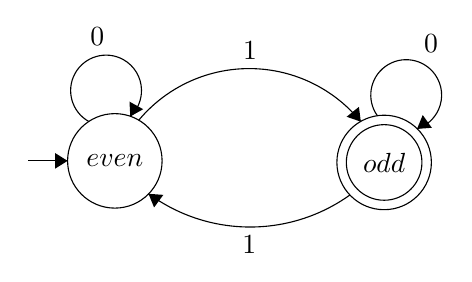
\begin{tikzpicture}[scale=0.2]
\tikzstyle{every node}+=[inner sep=0pt]
\draw [black] (19.9,-30.1) circle (3);
\draw (19.9,-30.1) node {$even$};
\draw [black] (37,-30.2) circle (3);
\draw (37,-30.2) node {$odd$};
\draw [black] (37,-30.2) circle (2.4);
\draw [black] (14.4,-30.1) -- (16.9,-30.1);
\fill [black] (16.9,-30.1) -- (16.1,-29.6) -- (16.1,-30.6);
\draw [black] (21.412,-27.525) arc (140.17246:39.15742:9.139);
\fill [black] (35.52,-27.61) -- (35.4,-26.67) -- (34.62,-27.3);
\draw (28.49,-23.73) node [above] {$1$};
\draw [black] (34.833,-32.261) arc (-54.34436:-126.32576:10.882);
\fill [black] (22.04,-32.19) -- (22.39,-33.06) -- (22.98,-32.26);
\draw (28.43,-34.81) node [below] {$1$};
\draw [black] (36.578,-27.242) arc (215.85773:-72.14227:2.25);
\draw (39.98,-23.25) node [above] {$0$};
\fill [black] (39.09,-28.07) -- (40.03,-28) -- (39.45,-27.19);
\draw [black] (18.256,-27.605) arc (241.11611:-46.88389:2.25);
\draw (18.79,-22.81) node [above] {$0$};
\fill [black] (20.88,-27.28) -- (21.7,-26.82) -- (20.83,-26.34);
\end{tikzpicture}
\end{center}



\definition{A \textbf{deterministic finite automaton (DFA), $M$, is a 5-tuple $(Q,\Sigma , \delta , q_0, F)$.}
	\begin{enumerate}
		\item[] $Q$, the set of states.
		\item[] $\Sigma$, the alphabet
		\item[] $\delta:Q\times\Sigma\rightarrow Q$, the transition function
		\item[] $q_0$, the start state
		\item[] $F$, the accept states
	\end{enumerate}
	
	
\definition{$M$ \textbf{accepts} a string $s=s_1 s_2 \dots s_k$ if there is a sequence of states in $M$ starting with $q_0$ and ending in a final state $q_0 q_1 \dots q_k$ such that $\delta(q_i,s_{i+1}) = q_{i+1}$.}

\definition{If $\mathcal{L} = \{s | M \ accepts \ s\}$, the we say $M$ \textbf{recognizes} $\mathcal{L}$.}
\definition{If a language $\mathcal{L}$ is recognized by some DFA, then it is \textbf{regular}.}

\definition{A \textbf{nondeterministic finite automaton (NFA), $M$, is a 5-tuple $(Q,\Sigma , \delta , q_0, F)$.}
	\begin{enumerate}
		\item[] $Q$, the set of states.
		\item[] $\Sigma$, the alphabet
		\item[] $\delta:Q\times \Sigma\cup\{\epsilon\}\rightarrow\mathcal{P}(Q)$, the transition function
		\item[] $q_0$, the start state
		\item[] $F$, the accept states
	\end{enumerate}
	
	Now, $\delta$ maps the current state and input character or $\epsilon$ to some subset of states.

\definition{A string $s$ is \textbf{accepted} by and NFA $M$ if there is some path for $s$ from the start state to a final state.}
\definition{$M$ \textbf{recognizes} a language $\mathcal{L}$ consisting of all strings it accepts.}

Example: let $\mathcal{L} = \{s|the 3rd \ last \ character \ is \ a \ 1\}$.


\begin{center}
	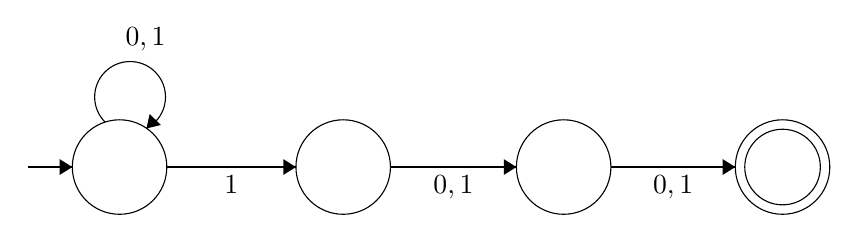
\begin{tikzpicture}[scale=0.2]
	\tikzstyle{every node}+=[inner sep=0pt]
	\draw [black] (10.6,-28.6) circle (3);
	\draw [black] (24.8,-28.6) circle (3);
	\draw [black] (38.8,-28.6) circle (3);
	\draw [black] (52.7,-28.6) circle (3);
	\draw [black] (52.7,-28.6) circle (2.4);
	\draw [black] (4.8,-28.6) -- (7.6,-28.6);
	\fill [black] (7.6,-28.6) -- (6.8,-28.1) -- (6.8,-29.1);
	\draw [black] (13.6,-28.6) -- (21.8,-28.6);
	\fill [black] (21.8,-28.6) -- (21,-28.1) -- (21,-29.1);
	\draw (17.7,-29.1) node [below] {$1$};
	\draw [black] (27.8,-28.6) -- (35.8,-28.6);
	\fill [black] (35.8,-28.6) -- (35,-28.1) -- (35,-29.1);
	\draw (31.8,-29.1) node [below] {$0,1$};
	\draw [black] (41.8,-28.6) -- (49.7,-28.6);
	\fill [black] (49.7,-28.6) -- (48.9,-28.1) -- (48.9,-29.1);
	\draw (45.75,-29.1) node [below] {$0,1$};
	\draw [black] (9.69,-25.754) arc (225.46923:-62.53077:2.25);
	\draw (12.25,-21.26) node [above] {$0,1$};
	\fill [black] (12.31,-26.15) -- (13.22,-25.93) -- (12.51,-25.23);
	\end{tikzpicture}
\end{center}





















